\subsection{State of the Art}
Indenfor skemalægning findes allerede nogle løsninger på de udfordringer, som kan opstå indenfor skemalægning. Et af disse er USA Schedulers' program kaldet School Master Scheduling Software\cite{USAS}, et program som først og fremmest tager de studerende i betragtning. Programmet er i stand til at lave funktionelle skemaer ud fra de studerenes ønsker, analysere de mest optimale løsninger ud fra ønskerne, og ud fra dette undgå konflikter så som 2 moduler, der ligger samtidigt, så studerende, der deltager aktivt i begge, bliver nødt til at vælge den ene fra.

Et andet stykke software kaldet Mimosa Scheduling Software\cite{Mimosa}, fokuserer mere på de grundlæggende udfordringer så som overbooking og nemt at kunne ændre på skemaerne, hvis der skulle komme en uventet udfordring. Det er i stand til at lave skemaer for lærere, elever, klasser og lokaler, alt det som enhver dansk folkeskole har brug for. Institutionerne henter programmet, laver deres egne ressourcer, hvilket vil sige lærere, elever, lokaler osv. og fordeler derefter de forskellige ressourcer ud over dagene. Programmet vil så fortælle, om dette kan lade sig gøre, og hvis dette ikke er tilfældet, vil det fortælle hvorfor\cite{MimosaTutorial}. I modsætning til School Master Scheduling, er Mimosas program mere henvendt til skemalæggerne og ikke så meget til de studerende. 

Begge programmer løser dog så at sige ikke selve skemalægningsopgaven, da dette stadig gøres manuelt af skemalæggeren eller de individuelle studerende for deres eget skema, men fungerer i stedet som et kontrolerende led. Ser man på de 10 mest anbefalede skemalægningsprogrammer fra hjemmesiden TopTenReviews\cite{top10Schedulers}, er de ikke rangeret ud fra automatisk skemalægning. Programmet som kommer tættest på, vil være Auto-Scheduler, men denne funktionalitet virker kun for medarbejdere ud fra en historik og er derfor ikke automatisk skemalægning. Besøger man et af de ti anmeldte programmers hjemmesider, finder man ingen information omkring programmernes evner indenfor dette. Et program som vil være i stand til helt automatisk at lave skemaer til alle på for eksempel en dansk folkeskole, udelukkende ud fra information om de ansatte, eleverne og tilgængelige klasselokaler, vil derfor være innovativt og nyttigt. Disse top-ti skemalægningsværktøjer er også mest henvendt til firmaer, så firmaerne kan tildele hver lønmodtager, arbejdsopgaver og holde styr på, hvor meget løn hver lønmodtager får, hvilket er noget anmeldelsesiden går meget op i og bedømmer skemalægningsværktøjerne ud fra.

På Tingstrup skole vil et program ved navn Tabulex blive taget i brug i forbindelse med skemalægningen. Det er et skemalægningsværktøj, der som de forrige kræver at brugeren stiller programmet en hel del krav, heriblandt hvordan lærerens tid skal prioriteres, hvornår lektionerne ligges, og hvor meget hver af disse regler skal prioriteres og overholdes af programmet\cite{Tabulex}. Tabulex kan selv forsøge i bedste fald, at lægge et skema ud fra de mange begrænsninger, som skemalæggeren har stillet programmet, og undervejs vil det informere brugeren, hvis kravene som er opstillet ikke muliggør et skema og man kan rette dem til. Herefter er det  muligt at fortsætte lægningen, eller starte lægningen forfra. Ligesom de andre skemalægningsværktøjer, kommer det med en grafisk brugerflade, som understøtter drag\&drop, og som er rimelig overskuelig. Tabulex kan dog ikke holde styr på regnskabet ligesom værktøjerne i forhenværende afsnit, men dette er heller ikke hvad programmet er lavet til at håndtere. Udover dette har Tabulex en fin dokumentation omkring hvordan programmet eksporterer til en .csv fil\cite{Tabulex_csv}, og da et af kravene stillet af vores case er, at det endelige skema skal kunne inddrages i Skoleintra, KMD Elev og andre programmer,\cite{interview_Kaerby} som netop tager imod .csv-formatet, er dette noget vi vil kigge nærmere på.
\begin{figure}[h!]
	\centering
	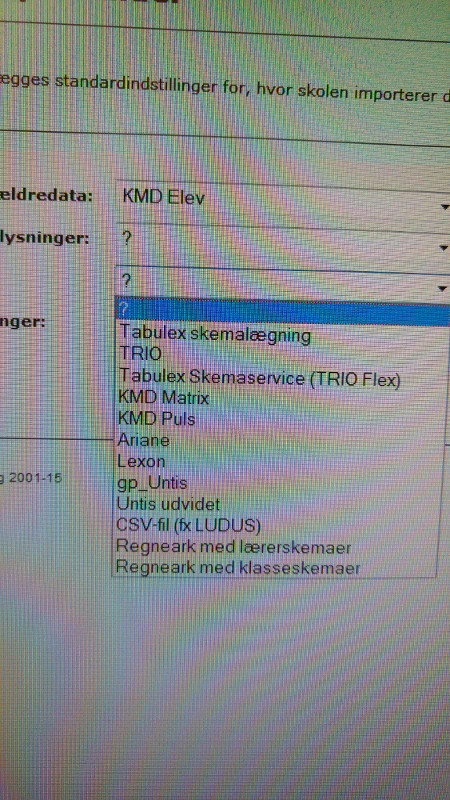
\includegraphics[width=0.4\textwidth]{../Billeder/Skemaimportering_filtyper_Intra.jpg}
	\caption{Skolens online system SkoleIntra kan læse forskellige filformater}
	\label{fig:kompatibleFiltyper}
\end{figure}
\FloatBarrier
Et andet program Tingstrup-skolen brugte, er KMD Educa, hvilket er en samling af forskellige værktøjer\cite{KMD}, der gør det muligt blandt andet at vikarføre, lægge skemaer og håndtere karakterresultater for den enkelte elev, som går på skolen eller har gået på skolen. Dette er en af de mange grunde til, at Aalborg Kommune har valgt at benytte sig af KMD Educa programmet ``Elev''\cite{useCase_KMD_Educa_Elev}.

Vores case, Kærbyskolen, brugte et program kaldet Docendo før skolestart 2015, men selvom firmaet selv giver udtryk for, at deres program er meget fleksibelt\cite{Docendo}, var det ikke fleksibelt nok for skolen og de valgte derfor at ligge skemaet manuelt. Programmet tillader at lægge skemaet elektronisk, lave varierende lektionslængde og tælle brugte timer, så eleverne hverken får for lidt lektioner, eller alt for mange. Ud fra deres video\cite{Docendo_video}, er det nemt at gå til, klasserne kan holdes styr på i en grafisk brugerflade, lektionerne kan flyttes rundt som det passer en, og hvis man gør dette, ændres tidspunktet i lektionsrubrikken også. Skemaet lægges dog for hver uge, men dette er i sidste ende ligegyldigt, da den tidligere uges skema godt kan genbruges.
